\section{Results}\label{sec:results}
    To validate this new feature, we performed a parameter scan study on a PWR
    pincell geometry.  Table \ref{tab:mat-params} contains the material
    parameters of our model, and Table \ref{tab:geo-params} contains the
    geometric parameters.

    We used the ENDF/B-VII.1 nuclear data library available at
    \url{openmc.org/official-data-libraries}. We used the ENDF/B-VII.1 depletion
    chain in the PWR spectrum available at \url{openmc.org/depletion-chains}.
    
    \begin{table}
        \caption{Material Parameters}\label{tab:mat-params}
        \begin{tabular*}{\tblwidth}{|c|c|c|c|}
            \hline
             Item & Fuel & Cladding & Water \\ % Table header row
            \hline
             Density [g/cc] & 10.4 & 6 & 1.0\\
             Volume [cc] & 0.1764$\pi$ & & \\
             S($\alpha$,$\beta$) &  & & \verb.c_H_in_H2O.\\
            \hline
        \end{tabular*}
    \end{table}
    
    \begin{table}[<options>]
        \caption{Geometric Parameters}\label{tab:geo-params}
        \begin{tabular*}{\tblwidth}{|c|c|c|}
            \hline
            Fuel Radius & Clad Radius & Water Bounding Box dimensions\\
            \hline
            0.42 & 0.45 &  1.24 $\times$ 1.24\\
            \hline
        \end{tabular*}
    \end{table}


    We used timestep size, depletion timestepper, and normalization method as
    our parameters to vary.

    Table \ref{tab:timestep-shorthands} shows the different timestep sizes we
    used and their shorthand terminology. All simulations ran for 10 depletion
    steps.

    \begin{table}[<options>]
        \caption{}\label{tab:timestep-shorthands}
        \begin{tabular*}{\tblwidth}{@{}LL@{}}
            \toprule
            Timestep sizes & Shorthand term \\ % Table header row
            \midrule
            360 seconds & Minutes\\
            4 hours & Hours\\
            3 days & Days\\
            30 days & Months\\
            \bottomrule
        \end{tabular*}
    \end{table}
    
    We used two different depletion timesteppers: \verb.PredictorIntegrator.,
    analagous to Gauss' method, and \verb.CECMIntegrator., a predcitor-corrector
    extension of Gauss' method.

    The last parameter, determines how neutron flux is calculated, and we also
    had two values for this: \verb.fission-q. normalization, and
    \verb.source-rate. normalization. \verb.fission-q. normalization uses
    fission Q  values in the depletion chain to calculate the flux. For the
    \verb.IndependentOperator. class, the equation used to calculate the flux
    using fission Q values is

    \begin{equation}
        \bar{\phi'} = \frac{P}{\sum\limits_i (Q_i \bar{\sigma}^f_i N_i)}
    \end{equation}

    where $P$ is the power, $Q_i$ is the fission Q value for nuclide $i$,
    $\bar{\sigma}_i^f$ is the one-group microscopic fission cross section for
    nuclide $i$, and $N_i$ is the number of atoms of nuclide $i$.

    \verb.source-rate. normalization uses a constant flux value to calculate the
    reaction rates. We caclulated the flux based on the initial material
    composition of the PWR pincell to be 1164719970082145.0 n/cm$^2$-s

    For each parameter combination, we ran with three cases:
    \begin{enumerate}
        \item Transport-coupled depletion
        \item Transport-independent depletion
        \item Transport-independent depletion with microscopic cross sections
            updated after each depletion step.
    \end{enumerate}

    For the first case, we used 25 inactive and 125 active batches, with 1e6
    particles per batch.

    We wrote a custom script to run the the third case. It should be noted that
    the third case is significantly slower than using transport-coupled depletion
    as the cross sections need to be reloaded after each depletion step due to how
    we wrote the script.

    Three cases and 16 parameter combinations gives 48 simulations total. All
    depletion simulations used a linear power density of 174 W/cm.

    To avoid a prohibitvely long paper, we will only show a subset of the
    results for each parameter. Unless otherwise specified, all results are
    using 3 day timesteps, \verb.fission-q. normalization, and
    \verb.PredictorIntegrator.  The general trend is that errors are smaller for
    shorter depletion timesteps, and larger for longer depletion timesteps.
    Interested readers can find the full results -- including figure geneartion
    scripts for all cases --  \ldots

    %TODO: Get the external data repo set up!!

    % actinides error 

    \begin{figure}[h!tpb]
        \centering
        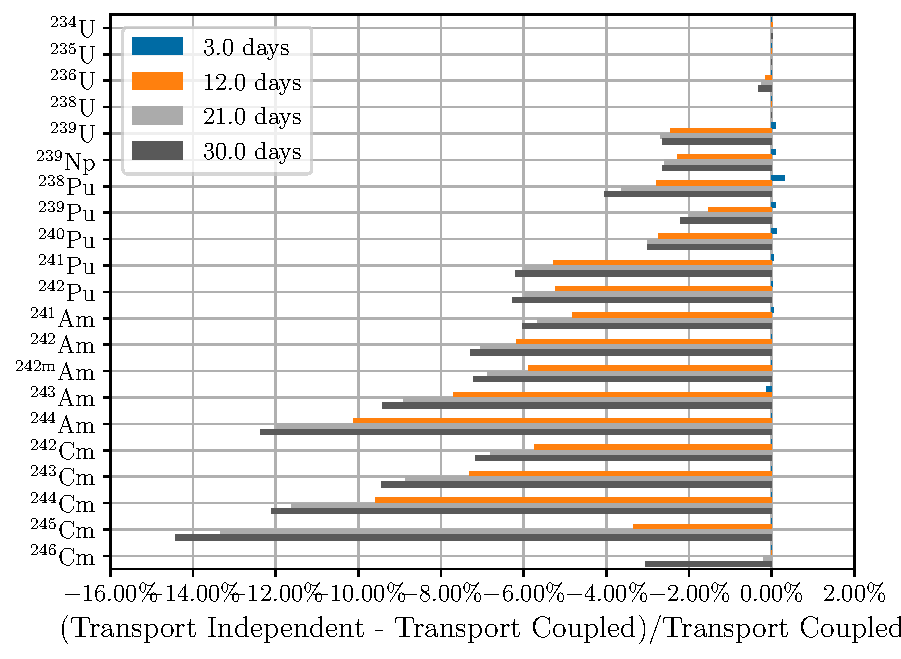
\includegraphics[width=\linewidth]{figs/actinides_constant_xs_predictor_fission_q_days.pdf}
        \caption[]{Actinide error in the fuel using constant cross sections.}
        \label{fig:actinides-error-constant-xs}
    \end{figure}

    Figures \ref{fig:actinides-error-constant-xs} and
    \ref{fig:actinides-error-updating-xs} show the relative error for actinides
    using constant cross sections and updating cross sections, respectively.  As
    expected, updating the cross sections at each depletion step results in very
    low errors, on the order of a fraction of a percent.  Using constant cross
    sections, the errors may be very low (5\% or less) or very high (more than
    10\%) depending on the nuclide of interest.

    \begin{figure}[htpb]
        \centering
        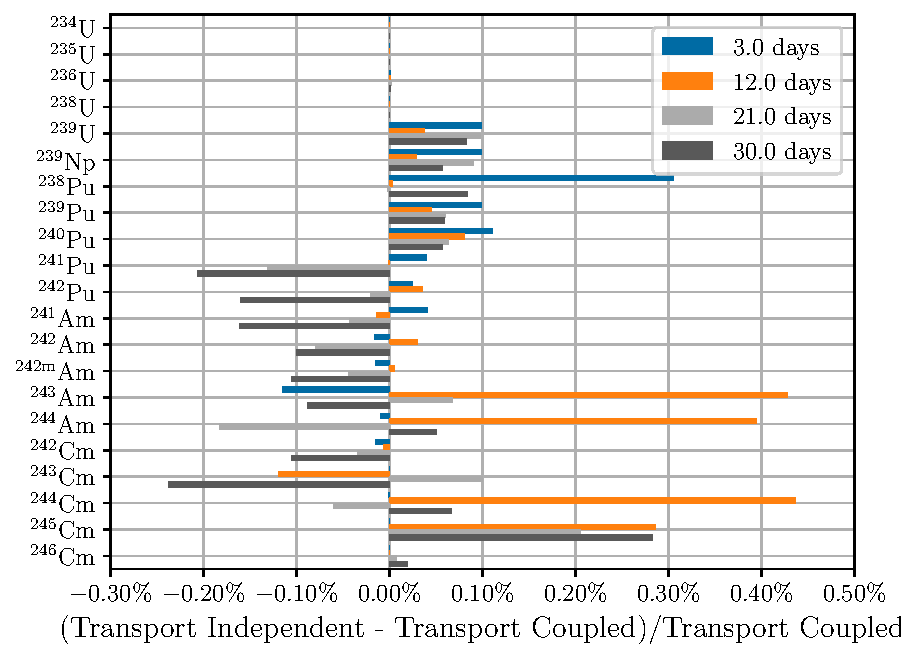
\includegraphics[width=\linewidth]{figs/actinides_updating_xs_predictor_fission_q_days.pdf}
        \caption[]{Actinide error in the fuel using updating cross sections}
        \label{fig:actinides-error-updating-xs}
    \end{figure}
    
    We suspect that the errors for isotopes of \ce{Am} and \ce{Cm} are so high
    are due to their extremely low composition in the fuel.
    %expand on this?


    % fission products error

    \begin{figure}[h!tpb]
        \centering
        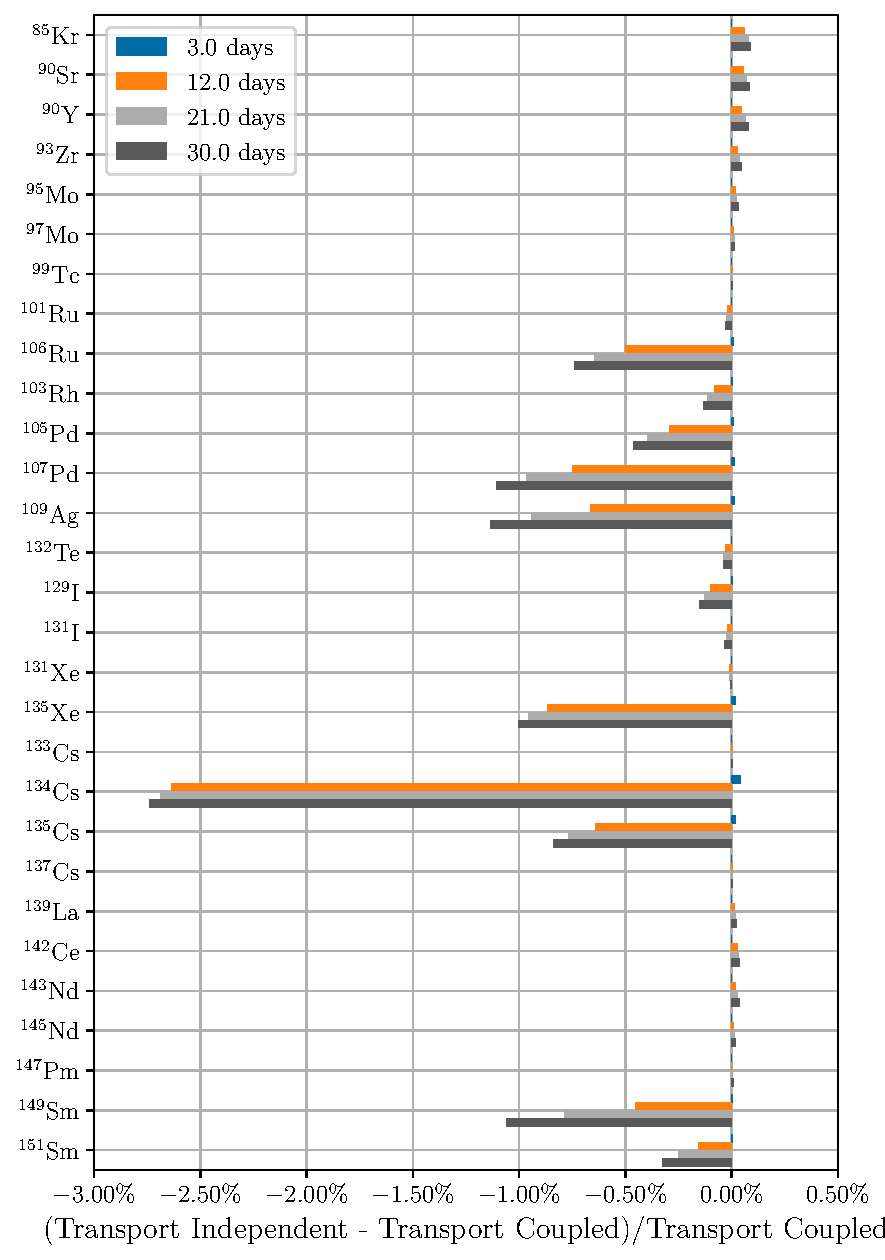
\includegraphics[width=\linewidth]{figs/fission_products_constant_xs_predictor_fission_q_days.pdf}
        \caption{Fission product error using constant cross sections}
        \label{fig:fp-error-constant-xs}
    \end{figure}

    Figures \ref{fig:fp-error-constant-xs} and \ref{fig:fp-error-updating-xs}
    show the relative error for fission products using constant cross sections
    and updating cross sections, respectively.

    Similar to the actinides, updating the cross sections at each depletion step
    results in errors in the nuclide compositions  that are fractions of
    percents. However, unlike the actinides, the errors when using constant
    cross sections are all relavtively low, with the largest error being under
    3\%. A majority of our fissile material is uranium, specifically
    \ce{^{235}U}, and the error for that nuclide is so low that it doesn't even
    show on Figure \ref{fig:actinides-error-constant-xs}. It follows that the
    majority of our fission products come from \ce{^{235}U} in a composition
    that is equally low in error. The other actinides are present in amounts
    with higher error, but in very low quantities, so their effect on the error
    of the fission product compoistions is proportionaly small.
    
    \begin{figure}[htpb]
        \centering
        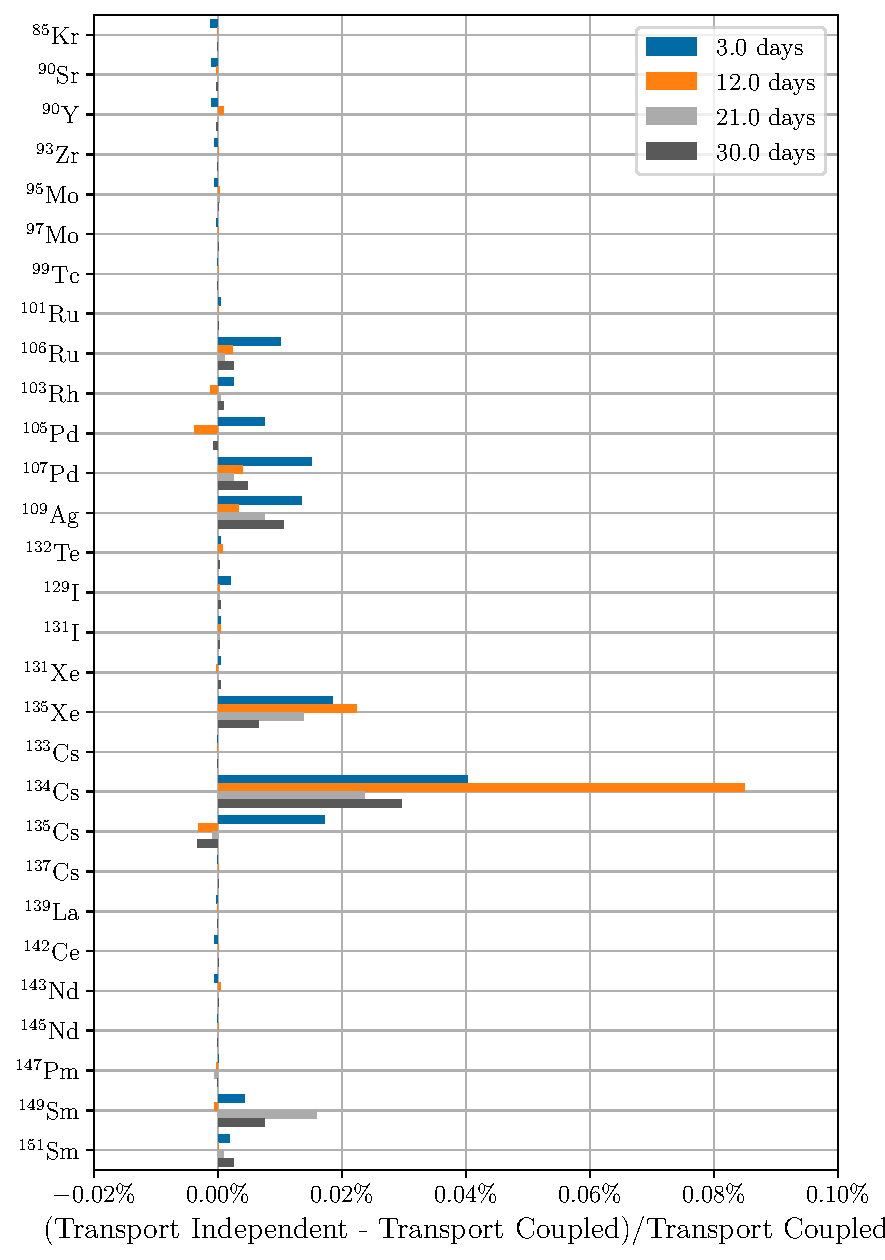
\includegraphics[width=\linewidth]{figs/fission_products_updating_xs_predictor_fission_q_days.pdf}
        \caption{Fission product error using  updating cross sections}
        \label{fig:fp-error-updating-xs}
    \end{figure}

    \begin{figure}[htpb]
        \centering
        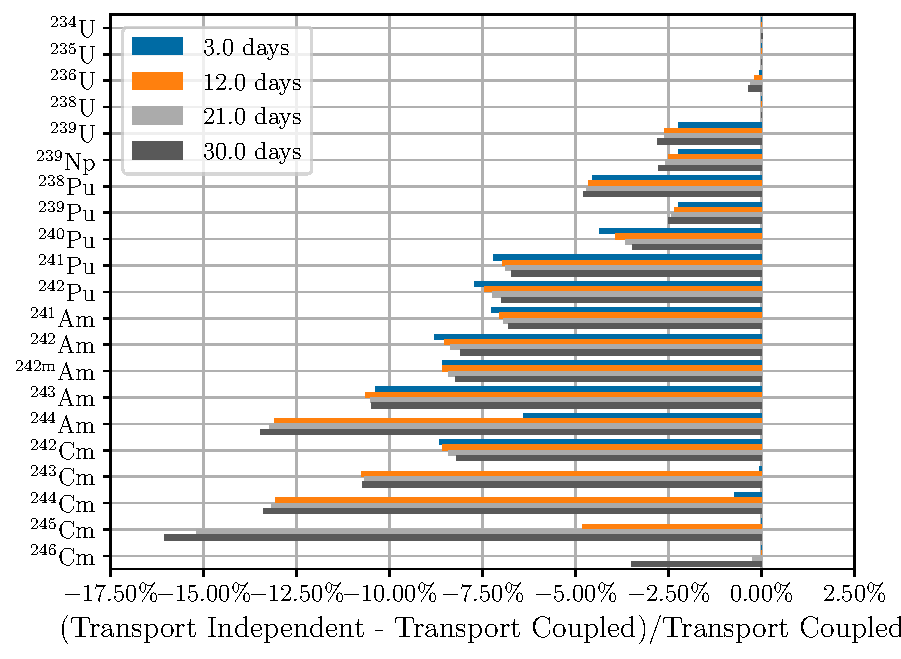
\includegraphics[width=\linewidth]{figs/actinides_constant_xs_cecm_fission_q_days.pdf}
        \caption{Actinide error using the CECM integrator}
        \label{fig:actinides-error-cecm}
    \end{figure}


    % actinides predictor vs cecm
    Figure \ref{fig:actinides-error-cecm} shows the error for actinides using the
    \verb.CECM. integrator. Comparing these results with those of Figure
    \ref{fig:actinides-error-constant-xs} we do not see a significant difference
    in the error. For certain nuclides, the \verb.CECM. integrator appears to
    perform worse. We see a similar pattern for the fission products.

    \begin{figure}[htpb]
        \centering
        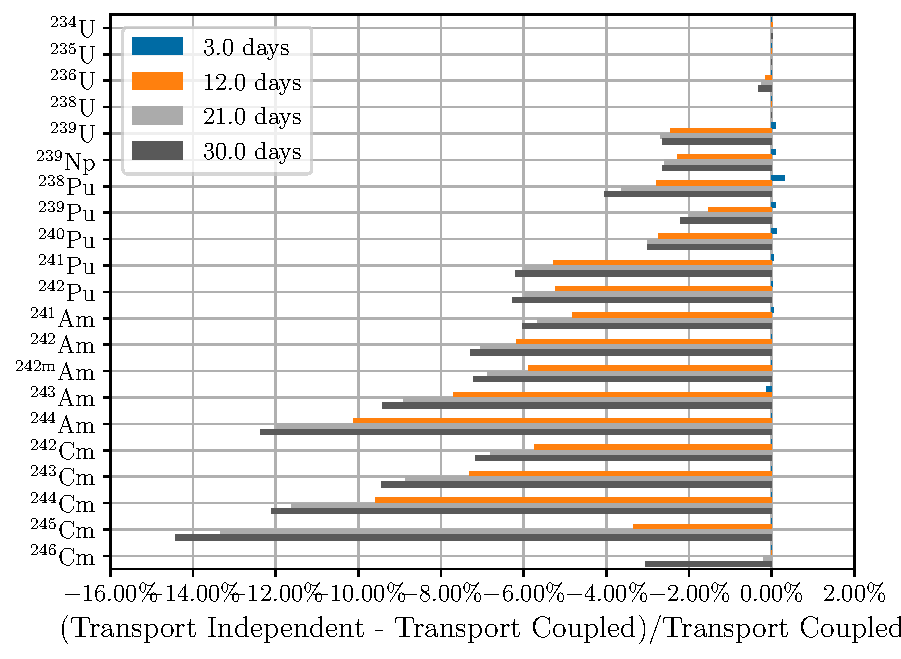
\includegraphics[width=\linewidth]{figs/actinides_constant_xs_predictor_source_rate_days.pdf}
        \caption{Actinide error using explicit value for the flux}
        \label{fig:actinides-error-source}
    \end{figure}

    Figure \ref{fig:actinides-error-source} shows the error for actinides using
    the flux we calculated from the initial material composition. These results
    do not differ significantly from the results in Figure
    \ref{fig:actinides-error-constant-xs}. The same is true for the fission
    products.

    Finally, a word on runtime; unfortunately, a bug present in the code during
    our study prevented collection of exact runtimes that would normally be
    stored in the statepoint files. Based on our time developing and testing
    this code, as well as running the simulations, the time savings when using
    \verb.IndependentOperator. are immense. Whereas the transport-coupled
    simulations each took several hours to complete, the transport-independent
    simulations took seconds to minutes to complete!


